\section{Introduction to Bitcoin}
When we need to buy something on the web typically we use the SSL protocol and a credit card. This approach is very simple, because doesn't need any specialized software, it's compliant with the credit card mechanism and it's one of the most used method for paying in the web. However, using this approach we reveal our information to potential malicious sellers and these increases the number of possible disputes. Furthermore, this approach is an expensive method for the shop that sells the the item of interest of the user and for sure the transaction for buy such item is not anonymous but is correctly tracked by the credit card company. For this reason, many credit card companies proposes a mechanism called \textbf{Secure Electronic Transactions (SET)}. We want to underline that this system never became operative for several reasons : all users must have a certificate for guaranteeing their payments and was too complex to put in place from the requirements standpoint both for shops and users. Few years later Satoshi Nakamoto developed \textbf{Bitcoin (BTC)}, which is a digital coin that beyond the money characteristics has the two following additional properties : it's decentralized (absence of a central authority) and it's immune to sovereign censorships. We can see Bitcoin as a combination of a currency, a payment system and a collection of algorithms and software implementation. The primary goal of the Bitcoin inventor was to make a system with low transaction costs and anonymous. In march $2017$ one bitcoin is worth about $\$ 1141$. There are slightly more $15$ million bitcoins, but the algorithm has been implemented in such a way that won't be no more than $21$ million bitcoins if the protocol doesn't changes. Now the question is how can we use Bitcoin ? First of all we need to visit \textit{bitcoin.org} website, and we create a wallet which has associated an ID. Then using a proper software for managing our wallet, it will create public/private key pairs for us as needed. For each pair, there is a corresponding bitcoin address, which is a $160$-bit hash of the public key. Then we send the bitcoins to the recipient address and we sign the transaction with our private key, so that the recipient can check our identity. Notice that a transaction might also include a small transaction fee. Bitcoin uses the following cryptographic tools :
\begin{itemize}
\item \textbf{Hash functions} : its input can be any string of any size and produces in an efficient way a fixed size output. In particular, for a hash function we requires the following properties :
\begin{itemize}
\item \textbf{Collision-resistance} : a hash function $H$ is said to be collision resistance if it's infeasible to find two values $x$ and $y$  with $x \neq y$ s. t. $H(x) = H(y)$.
\item \textbf{Hiding} : a hash function $H$ is hiding if, when a value $r$ is chosen from a probability distribution that has high min-entropy, given $H(r \mid x)$ it's infeasible to find $x$.
\item \textbf{Puzzle friendliness} : a hash function $H$ is said to be puzzle-friendly if for every possible $n$-bit output value $y$ and for $k$ chosen from a distribution with high min-entropy, then it infeasible to find $x$ such that $H(k \mid x) = y$ in time significantly less than $2^{n}$.
\end{itemize}
\item \textbf{Digital signatures} : 
\item \textbf{Public key} :
\end{itemize}
Bitcoin is based on the concept of \textbf{search puzzle}. A search puzzle consist of a hash function $H$, a value id with represent the puzzle-ID chosen from a high min-entropy distribution and a target set $Y$. A solution of the search puzzle is a value $x$ such that $H(id \mid x) = Y$. If a search puzzle is puzzle-friendly then there is no solving strategy for this puzzle which is much better than just trying random values of $x$. Now, we want to understand why designing a electronic cash is so hard. The first issue that we could face goes under the name of \textbf{double spending}. Suppose Alice that has $X$ bitcoins and sends a message to Bob says "ok, transfer $X$ bitcoins to Bob". Next, Alice at the same time sends also a message to Charlie to transfer to him the same amount of bitcoins. In other words Alice is trying to double spending its $X$ bitcoins. Now, if there is a bank for handling this problem is very easy, but at this point we are at the starting point again because the bank knows everything and it's working for us and should be paid. A possible solution to avoid this problem is to maintain a block chain as a public ledger of all transactions. So when Alice wants to adds a block to this ledger for sending $X$ bitcoins to Bob, the operation is permitted. Whereas, when Alice in a future time point, will try to add a block correspondent to the transactions towards Charlie, the operation will not be allowed, because there is a check that notice that Alice is not the owner of such amount of bitcoins anymore. Typically in bitcoin, each block contains several transactions and a new one is created every $\sim 10$ minutes. Naturally each block should be coherent, i.e. coherence means that two transactions for the same amount of bitcoins from the same user should belongs to the same block, otherwise the Bitcoin community will easily notice that that user is trying to double its bitcoins. So the idea is to make this public ledger as the central authority for managing and checking all the transactions. The block chain used by Bitcoin is a sequence of blocks connected by hash function. The idea is that the last block contains data (transactions done in the last $10$ minutes) plus the hash of the previous block. Naturally, the previous block contains data plus the hash of the previous block as well. The idea of using a block chain for managing transactions is that if an adversary modifies data anywhere in the block chain, it will result in the next hash pointer being incorrect and we are going to detect it. If we store the head of the list and even if the adversary modifies all the pointers in order to be consistent with the modified data, the head pointer will be incorrect, and we will detect the tampering. However, the usage of a block chain doesn't guarantee us the truth, but preserve truth and lies from later alterations, allowing to securily analyze them and be more confident in uncovering the lies. We know that a user in the Bitcoin network are characterized by a public key, which digest is called \textbf{address} in Bitcoin jargon. Now, we want to see two attempts about the issue of double spending :

\paragraph{Goofy coin} The first rule is that a designated entity called Goofy, can create new coins whenever he wants and these newly created coins belong to him. To create a coin, Goofy generates a unique coin ID that he's never generated before to be assigned to the coins previously created. At this point, he computes the digital signature for such coins using its secret key, so that everybody can verify that the coin contains a valid signature or not. Now, suppose Goofy wants to transfer a coin that he created to Alice. To do this he creates a new statement that say "Pay $X$ coins to Alice", where $X$ represent the amount of coins to be transferred to Alice. We recall that identities are just public keys, so Alice refers to Alice's public key. Finally, Goofy signs the string representing the statement. Everybody in the network can verify the transaction signature using the Goofy public key associated with the private key used for signing the transaction itself, and if it's valid then we can say that an amount of $X$ coins has been transferred from a person to another person. At the end, everybody knows that such amount of coins are owned by Alice and not anymore by Goofy. However, this approach doesn't avoid Alice from double spending its own coins.

\paragraph{Scrooge coin} Another approach is to use a centralized entity named Scrooge that publishes the history of all transactions that have happened. To do this it uses a block chain digitally signed by itself. In such a way everyone can verify if :
\begin{itemize}
\item the coins are valid, which means that they were really created in previous transactions.
\item the coins were not already consumed in some previous transaction, i.e. it's not double-spending.
\item the total value of the coins that come out of this transaction is equal to the total value of the coins that went in. In other words, only Scrooge can create new value.
\item the transaction is validly signed by the owners of all the consumed coins.
\end{itemize}
In this case we need to trust Scrooge about the transactions. For this reason, if all the previous conditions are met, then the transaction will be accepted by Scrooge. In particular, Scrooge write the transaction into the history by appending it to the block chain, so that everyone can see that a new transaction occurred. In this way we avoid the double spending issue, because it's only when Scrooge publishes the transaction that the other users can accept that the transaction has actually occurred. However there are two problems with this approach : there is one person that is responsible for everybody and that we delegate one person to be in charge of everything. In other words, we need to trust Scrooge that is honest, but this represent a weakness since it can be attacked.\\\\Another system that is trustable like Scrooge coin but doesn't have a central authority is Bitcoin. However, due to the absence of a central authority, in such system is very hard to reach consensus. Indeed a distributed consensus protocol has the following two properties : it must terminate with all honest nodes in agreement on the value, and the value must have been generated by a honest node. Essentially, when Alice send a message to Bob for paying him, she broadcast the transaction to all Bitcoin nodes that comprises the peer-to-peer network. In Bitcoin network we have the following consensus requirements :
\begin{itemize}
\item \textbf{Many users broadcast transactions} : the nodes must agree on exactly which transactions where broadcast and the order in which these transactions happened.
\item \textbf{Many ledgers} : at any given point, all the notes in the peer-to-peer network have a ledger consisting of a sequence of blocks, each containing a list of transactions, that they have reached consensus on.
\item \textbf{Keep consistency} : all nodes agree on a single global ledger for the system.
\end{itemize}
When a block is proposed by a node with a ledger, all the other nodes executes some consensus protocol in order to check if such block is correct or not. To propose a block to the community we need to solve a search puzzle, which is hard to solve. If the block is correct (you solved the puzzle) the block is accepted and you will receive a reward for it. However, at the same time there may be two people that propose correct blocks, but at that point there is some consensus protocol that decides which of the two blocks needs to be accepted. The problem with this approach is that the network is not perfect and for this reason there could be latency and crashing nodes or malicious nodes that try to subvert the process. Bitcoin consensus overcome the main problems of the traditional consensus models using two tricks : nodes receives rewards to be honest and that it uses randomization guaranteeing us that the probability of reaching consensus is overwhelmingly high. The consensus protocol used by Bitcoin can be summarized in the following way : first of all new transactions are broadcast to all nodes. Next, each node collects new transactions into a block and in each round a random node broadcast its block. The other nodes accept such block if and only if all the transactions inside it are valid. In positive case, the nodes express the acceptance of the block by including its hash in the next block they create. If there are more possibilities the node chooses the longest chain. The Bitcoin network can be subject to the so called \textbf{sybil attack}. In such case, the attacker creates several copies of nodes which are called \textbf{sybil}, so that they look like as a lot of different participants, when instead they are all controlled by the same adversary. Now the question is can we steal Bitcoins ? The answer is no, because if a miner proposes the next block stealing other user's bitcoins, would require the miner to create a valid transaction that spends that coin, which in turn means to forge the owner's private key to sign the transaction, but this cannot be done if a secure digital signature scheme is used. Another possible problem is the DoS attack, which comes from the fact that an user dislike another user. Suppose that $A$ doesn't like the user $B$. So $A$ can decide to not include any transaction originated from $B$'s address in any block that she proposes to get into the block chain, i.e. $A$ is denying the service to $B$. This may seems a valid attack, but if $B$'s transaction is excluded by the block proposed by $A$, he needs just to wait until a honest node gets the chance to propose a block and then his transaction will be inside that block. Now how does the double spending issue is avoided using Bitcoin ? Suppose Alice at the same time issues two payments with the same amount of Bitcoins towards two different addresses. The idea is that we need to kill one of these two transactions in order to avoid Alice from double spending its Bitcoins. In the procedure used for reaching consensus the nodes try to extend the transaction they are aware. The accepted transaction is the one that will be the longest, because nodes might be rewarded only by extending the longer chain. This is the reason why the Bitcoin community typically ignores the shorter chains, because in case of extending a shorter chain they might not be rewarded at all. Since the block containing the short transaction is ignored by the network, it's called an \textbf{orphan block}. Now the question is how long we have to wait to be sure that there is no double spending ? The intuition is that if we wait for more or less one hour, since a confirmation happens every $10$ minutes, we will expect to have around $6$ confirmations. Indeed, the number of confirmations provides confidence in the probability of the next accepted transaction and we have an exponential decrease in the probability of having a double spending issue. A node for computing a new block is required to find a nonce such that when it concatenate the nonce, the hash of the previous block, and the list of transactions that comprise that block and take the hash of such string, then such hash should be a number that falls into a target space that is quite small in relation to the much larger output space of that hash function. In particular, Bitcoin defines this target space as any value falling below a certain target value :
\begin{center}
$H(nonce \mid \mid previous\_hash \mid \mid tx \mid \mid ... \mid \mid tx) < target$.
\end{center}
Naturally, if the hash function chosen is good then accomplish this task is computationally hard (it requires computation power and time). This task refers to the fact of solving a hash puzzle. Obviously, they needs to be quite hard to compute. For example at the end of $2014$ the difficulty level for solving a hash puzzle was about $10^{20}$ hashes per block. We clearly understand that the size of the target space is only $\frac{1}{10^{20}}$ of the size of the output space of the hash function. The parameter of the difficulty is tuned on the basis on how many nodes are trying to create a new block every certain number of blocks by the protocol. This implies that if there are few nodes we will decrease the difficulty. Vice versa in presence of several competing nodes we will increase the difficulty. To do this the nodes in the Bitcoin network automatically recalculate the target every $2016$ blocks. In particular, they recalculate the target in such a way that the average time between successive blocks produced in the network is about $10$ minutes. With such average time between blocks, the $2016$ blocks can be processed in roughly two weeks, i.e. the target is recalculated every two weeks. For this reason only particular nodes with sufficient computing power capabilities can compete in this block creation process. This process of repeatedly trying and solving these hash puzzles is known as \textbf{Bitcoin mining}, and we call the participant nodes \textbf{miners}. The crucial point is that if we consider that the majority of miners are honest and follow the protocol then many attacks on Bitcoin are infeasible. This is true because if the majority of miners are honest, the competition for proposing the next block will automatically ensure that there is at least a probability of $\frac{1}{2}$ that the next block to be proposed comes from a honest node. Now the question is how long it will take a miner to find a block ? The average time for a miner to propose a new block is given by the ratio of $10$ minutes and the fraction of hash power that the miner has. For example, if the miner has the $0.1 \%$ of the total network hash power, find a block to propose every $10000$ minutes (about a week). To verify a block it's sufficient to check the hash of the block and that all transactions are correct. So, it's trivial that a node has computed the proof of work correctly. The nonce must be published as a part of the block, so that the other nodes can trivially verify that the output is less than the target. This is the reason why we don't need any centralized authority that verifies that miners are doing their job correctly. Furthermore, when a block is proposed there is a special transaction within in called \textbf{coin-creation transaction}, so that if the user that proposed the block is the lucky person that solved the puzzle than such user will give the coin just created to himself. We need to underline that this is the only way to create new coins and this is done in exchange to the work done for maintaining and proposing new blocks. The original reward was $50$, but it actually halves every $210000$ blocks. Halving every $210000$ blocks gives a geometric series, which gives us a finite sum of $21$ million Bitcoins.\\\\Nowadays proposing a new block is becoming more and more expensive. This implies that the reward that you have for a block might not be sufficient for paying all your expenses. The second issue is that the popularity of Bitcoin implies that there can be many requests to be processed an put in a block. Another Bitcoin requirement is that the size of a block cannot be very large. This implies that more or less we can have $200$ transactions in a block. If there are more than $200$ transaction and we want that our transaction is inside a block, we can insert in the transaction a small transaction fee to the miner that will include our transaction in the block. This is like paying a service offered by the miner, but it's not mandatory. In this way a miner that receives a transaction without a transaction fee and a transaction with a transaction fee, has an incentive to put the second transaction in the next block that he will propose. Naturally the costs of miners are given by hardware cost plus the electricity cost, and they have incentive to mine if and only if cost $<$ transaction fee $+$ block reward. We will expect that in $2040$ the block reward is $0$, and at this point we will really need transaction fees in our to allow Bitcoin to survive. We already said that the nodes in the Bitcoin network are not all equals. In general, we can distinguish two kinds of nodes :
\begin{itemize}
\item \textbf{Full nodes} : they are nodes that fully verify all the rules of Bitcoin and download the entire block chain. This type of nodes doesn't propose new blocks, but stores and answers to queries from other nodes. The full nodes main goal is to enforce the Bitcoin consensus rules. They have the following advantages :
\begin{itemize}
\item \textbf{Security} : running a full node is the only way we can use Bitcoin in a trustless way, because it will check that all the rules of the Bitcoin consensus protocol are satisfied.
\item \textbf{Privacy} : a full node is currently the most private way to use Bitcoin, with nobody else learning which Bitcoin addresses belongs to us.
\end{itemize}
\item \textbf{Light nodes} : they are nodes that don't download the complete block chain, but downloads the block headers in order to validate the authenticity of the transactions. For this reason, this type of nodes is easy to maintain and run. Typically light nodes are served by full nodes to connect to the Bitcoin network. However, they have some limitations such as :
\begin{itemize}
\item \textbf{Validation} : they don't validate the rules of Bitcoin. So if someone pays a light node with fake Bitcoins, then this latter will accept them and the user will be left out of its money.
\item \textbf{Privacy} : they typically send addresses to a trusted third party and receive the wallet balance and history. At that point the issue is that they are transferring all the information about the wallets that is more or less like a bank.
\end{itemize}
\end{itemize}
We understand that the light nodes doesn't check the Bitcoin consensus rules and for this reason can be tricked by everybody in the network, whereas full nodes check those rules and thus enforce the validity of the block chain itself. If there is a fake evolution of the block chain that contains for example a double spend transaction, then we may have a bifurcation of the block chain. This implies that that we will not have anymore a single Bitcoin community, but two Bitcoin communities each with its own currency. A direct consequence of such scenario is a decrease in the trust of Bitcoin, which will push people to abandon it and thus the value of Bitcoin will decrease as well. In practice, miners are unlikely to attempt the creation of such fork because as long as full nodes are prevalent they would lose a lot of money. To recap, it's critical for Bitcoin survival that the great majority of the Bitcoin economy be backed by full nodes.

\subsection{Bitcoin mechanics}
The transactions are not indicating transfer but ownership of coins. The bad point of such approach is that if someone wants to check if a transaction is valid then he needs to have the history of the transactions about the sender in order to check that at the time instant when the transaction has been triggered the sender has a balance greater or equal than the amount to transfer. A transaction is constituted by three components :
\begin{itemize}
\item \textbf{Metadata} : they represent information about the transaction such as its size, the number of inputs and the number of outputs. There is also the hash of the entire transaction which is used as a unique ID for the transaction.
\item \textbf{Inputs} : it's an array of inputs. Each input specifies a previous transaction (the hash of that transaction), the index of the previous transaction's outputs that being claimed and a signature.
\item \textbf{Outputs} : it's an array of outputs. Each output has just two fields : a value and the sum of all the output values that has to be less or equal than to the sum of all the input values.
\end{itemize}
In particular, Bitcoin offers the following services :
\begin{itemize}
\item \textbf{Change addresses} : typically when an user issue a transaction where its balance is greater than the amount of Bitcoins in the transaction itself, then he also issues a transaction also towards himself, because Bitcoins are immutable, hence the entirety of a transaction output must be consumed by another transaction.
\item \textbf{Efficient verification} : suppose that a new transaction is added to the public ledger. How easy is to check if it's valid ? We need to look up the transaction output that the user referenced, that it has a value of $6.25$ Bitcoins, and that it hasn't already been spent. To ensure it hasn't been spent, we need to scan the block chain between the referenced transaction and the latest block.
\item \textbf{Consolidating funds} : suppose that Bob has received money in two different transactions. If Bob wants to spend all the received money he just have to create a transaction with the two inputs and one output, with the output address being one that he owns, i.e. it's a way for allowing Bob to consolidate these two transactions.
\item \textbf{Joint payments} : it's a situation where a transaction has two or more inputs and a single output and it's signed by two or more people.
\item \textbf{Escrow transactions} : suppose that Alice wants to buy some item from Bob and she don't want to pay until she is sure to receive the object. To proceed Alice creates a MULTISIG transaction that requires two of three people to sign in order to redeem the coins : Alice, Bob and a third party Judy. So if there is no problem Alice and Bob sign and Bob can then use the coins. Otherwise in case of dispute, they call Judy as a judge to settle the issue.
\item \textbf{Green addresses} : suppose that Alice wants to pay Bob, but Bob is offline and thus cannot check if such transaction is actually there. For this reason, we introduce a third party to which Alice ask it to send the money to Bob. This third party takes the money from Alice and gives them to Bob. Naturally, this third party should be trusted also for checking double spending.
\end{itemize}
A Bitcoin block is structured in the following way : $4$ bytes for the block size, $80$ bytes for the block header, $1-9$ bytes for the transaction counter and a variable amount of bytes for all the transactions recorded in such block. Instead the block header is constituted by the following fields :
\begin{itemize}
\item \textbf{Version} (4 bytes) : it's a version number to track the protocol updates
\item \textbf{Previous block hash} (32 bytes) : it's a reference to the hash of the previous block in the chain
\item \textbf{Merkle root} (32 bytes) : it's the hash of the root of the merkle tree of the block's transactions
\item \textbf{Timestamp} (4 bytes) : it represent the approximate creation time of the block
\item \textbf{Difficulty} (4 bytes) : it's the proof-of-work algorithm difficulty target for the block
\item \textbf{Nonce} (4 bytes) : it's a counter used for the proof-of-work algorithm.
\end{itemize}
There is also a scripting language built on purpose for Bitcoin. It's very small (contains only $256$ no loop instructions). Clearly having only one transaction in a block is very slow because it will require a lot of work. So, the idea is to group several transactions per block. Now how can we check the validity of each single transaction ? A transaction doesn't know to which block it belongs. For this reason, Merkle trees are used to check if a transaction is in a block. A Merkle tree is a tree in which we have the data in its leaves, and in the internal nodes two hashes of the corresponding child nodes. In fact, a node to prove that a transaction is included in the block can simply produce a Merkle path that is only $4$ $32$ bytes hashes long. Now, how can we publish a transaction ? We can use a simple flooding algorithm that simply broadcast the transaction to all the nodes that are peered with us. Each of these nodes executes a series of checks to determine the validity of the transaction and in positive case the nodes in turn sends it to all of their peer nodes. Furthermore, when a node receives a transaction, it put the transaction in a pool of received transactions that aren't on the block chain yet. The propagation time of a block with a size of $200KB$ takes less than $30$ seconds to reach the $75 \%$ of the whole network. Now, we want to talk about an attack called \textbf{51-percent attack}. It's a scenario where an attacker controls the $51 \%$ or more of the mining power in the Bitcoin network. Even in this case, the attacker cannot steal coins from an existing address, because he needs to alter the sender signature but this would require him to break the cryptography. The attacker cannot neither suppress any user transactions, because a transaction is simply broadcast in the Bitcoin network and we are assuming that the attacker is not able to fully control the network. So, the transaction will reach the majority of nodes, that in turn, if the transaction is valid, will insert it in next block that they will propose. Finally, the attacker has a very low probability to be able to decrease the confidence of the Bitcoin network itself, because the cost of achieving a $51 \%$ majority really makes sense from a financial point of view.

\subsection{The miner role}
A miner has to follow a straightforward procedure in order to get a reward :
\begin{enumerate}
\item First of all the miner listen for transactions on the network and validate them by checking that signatures are correct and that the outputs being spent have not been spent before.
\item Next, he maintain the block chain and listen for new blocks. In particular, a miner before joining the network will ask to the other nodes all the historical blocks that are already part of the block chain. Next, he listen for new blocks that are being broadcast to the network. The miner must validate each block that receives by validating each transaction in the block and checking that the block contains a valid nonce.
\item Once the miner has an up-to-date copy of the block chain, he can begin building its own blocks. In order to do this, he group the transactions previously heard into a new block that extends the latest block he knows. Naturally the miner needs to make sure that each transaction included in its block is valid.
\item Then the miner needs to find a nonce that makes its own block valid. This is the most time and resources consuming step for him.
\item Once the miner have found a valid nonce, proposes a new valid block. However, the acceptance of such block is not guaranteed. So the miner needs to hope that other miners will accept its block and start mining in top of it, instead of some competitor's block.
\item If all miners accept the miner's block then he obtains the reward (in $2020$ the reward is $6.25$ BTC). In addition he collect the transactions fees of the transactions in its own block (today they represent only about $1 \%$ of block rewards).
\end{enumerate}
A transaction doesn't include a transaction fee if it's less than $1000$ bytes in size, all outputs are greater or equal to $0.01$ BTC, or priority is large enough. Otherwise a fee is charged and it's about $0.0001$ BTC for $1000$ bytes. We know that a miner is rewarded only on the basis on its hash computational power, but the problem is that he could be unlucky and doesn't get the reward at all. For this reason, a miner could merge its hash power with the ones of other miners in order to create the so called \textbf{mining pool}, in order to share the mining process costs.

\subsection{Getting a cryptocurrency}
Now we want to discuss how we can go from the Bitcoin protocol to a real digital money. The idea of having a digital currency requires three aspects : the security of the block chain, otherwise nobody will trust Bitcoin and nobody will use it, the health of the mining ecosystem, which means that if the miners don't get enough reward for their activities they won't do that for free and for this reason they may decide to not give computational power to maintain the system, and the value of the currency itself. When Bitcoin was first created, the previous three properties didn't hold. The critical point is that Bitcoin has not been proposed by a bank or a big company but by an unknown researcher known as Satoshi Nakamoto. Bitcoin is became so popular because the more people hear about it, the more they are going to get interested in mining and in turn this increases the confidence of people about the security of the block chain because there is now more mining activities going on, and so forth. Now the question is how can we maintain Bitcoins ? The simplest way is to store them on a local device such as a laptop. However, this requires to deal with Bitcoin secret keys. The problem is that if we lose the device or our file gets corrupted, our keys are lost and so are our coins. Furthermore, if somebody infects our device with a malware, then such person can copy our keys and then he can then send all our coins to himself. In general, we can store Bitcoins in the following two ways :
\begin{itemize}
\item \textbf{Hot storage} : it means that we store the Bitcoins on our computer, but this is very risky.
\item \textbf{Cold storage} : this approach works in offline mode. In particular, it's locked away somewhere and it isn't connected to the Internet. This approach is safer and more secure wrt the previous approach, but of course it's not convenient.
\end{itemize}
Naturally to have separate hot and cold storage we need to have separate secret keys, otherwise the coins stored in the cold storage would be vulnerable if the hot storage is compromised. A common scenario is to move coins between these two storage, which implies that both sides needs to know the address of the other one. The problem is that in such scenario we would like to use a fresh cold address for the money transfer. This can be done by generating a big batch of addresses all at once and give them to the hot storage in such a way when a money transfer is issued the hot side uses them up one by one. A more effective solution is to use a \textbf{hierarchical wallet}, which allows the cold side to use an unbounded number of addresses and the hot side will know about these addresses for performing the money transfers. However, these addresses will be available only for a short one-time communication between the two sides (to do that we need to use some cryptography trick). In particular, given an initial address generation information, there is a function that generates a sequence of public and private keys, which for any integer $i$ it generates the $i-th$ address and the $i-th$ secret key in the sequence. Obviously, knowing the list of public key doesn't reveal anything about 
any secret key.
\begin{center}
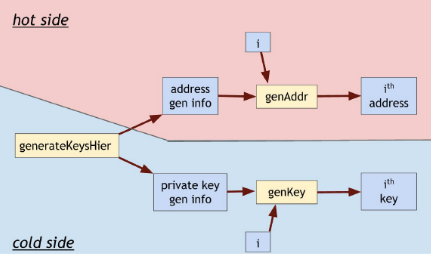
\includegraphics[scale=0.5]{./images/hierarchical_wallet_schema.png}
\end{center}
We understood that the ownership of BTC is given by knowing the keys and we must ensure that their retrieval is difficult. However, there are also other solution to store Bitcoins, such as \textbf{tamper resistant card} or \textbf{online wallet}. In the latter case, we give our keys to a trust entity, which acts like a bank and stores our Bitcoins. Another solution is to store Bitcoins in a \textbf{hardware wallet}. It represent a robust approach, but the users face the risk of losing access to their tokens if they misplace or forget their keys. A way to increase the security of the previous approaches is to use a \textbf{secret sharing mechanism}. Its main idea is to divide our secret key into some number $N$ of pieces and store them in several places, in such a way that if we are given any number $K$ of those pieces then we will able to reconstruct the original secret, but if we are given fewer than $K$ pieces then we won't be able to learn anything about the original secret. For example, suppose we have $N = 2 = K$. This means that we are generating $2$ shares based on the secret, and we need both shares to be able to reconstruct the original secret. Let's call our secret $S$ which is a $128$-bit number. We could generate a $128$-bit random number $R$ and make the two shares be $R$ and $S \oplus R$, i.e. we have use OTP schema. Next, we store the previous two shares in separate places. We can observe that neither the first nor the second share by itself tells us anything about the original secret $S$. Instead, if we have both shares we can simply XOR them in order to reconstruct the original secret. An interesting observation is that this trick works as long as $N$ and $K$ are the same, because we would just need to generate $N - 1$ different random numbers for the first $N - 1$ shares and the final share would be the XOR between the secret and all the others $N - 1$ shares. This means that if $N$ is greater than $K$, this doesn't work anymore and we need to use the algebra. For example, when $K = 2$ with $K < N$, then we can represent such schema in the 2D plane as a line with equation $y = k_{1}x + k_{2}$, where $k_{1}$ and $k_{2}$ represents the two shares. This means that if we know just two points of the line we can simply find the two shares, and thus we will be able to reconstruct the original secret. Naturally, this approach can be generalized in order to require $K > 2$ shares in order to be able to reconstruct the original secret.\\\\There are several kinds of entities that trades Bitcoins against flat currency like dollars and euros. In particular, we have :
\begin{itemize}
\item \textbf{Market users} : they are users that wants to use Bitcoins for privacy reasons. For example, they buy Bitcoins to perform transactions and then sell them.
\item \textbf{Investors} : they are users or companies that buy BTC to make money, with the hope that their value will increase for a possible future reselling.
\item \textbf{BTC intermediaries} : they are entities that simply sell and buy BTC, earning money by exchange fees.
\end{itemize}
The Bitcoin main advantage is \textbf{anonymity} but this is also a disadvantage, because allows both benign and malicious users to be anonymous. The price of Bitcoin will be set by supply and demand : the supply of Bitcoins that might potentially be sold and the demand for Bitcoins by people who have dollars/euros. Naturally if the demand decreases then the Bitcoin value will decrease as well, and increases in the other way around. Some economic models showed that the Bitcoin value depends also on the supply of BTC.

\subsection{Bitcoin anonymity}
For the anonymous word there can be two interpretations : without using our real name, and without using any name at all. Indeed in Bitcoin each user is specified by a public key which we typically call its \textbf{pseudo-identity}. The idea is that we do not know who physical person is behind that public key, but we know that over time the same person behind that public key will be the same person. However, anonymity is not sufficient for privacy but it's necessary. The problem is that in practice anonymity is unachievable. For this reason we will define anonymity as a combination of two aspects : pseudonymity and unlinkability. The first one we know what is, it's just the identity of a user represented by a public key. The second one expresses the fact that different interactions of the same user with the system shouldn't be linkable to each others. In particular, we reach unlinkability if the following properties holds :
\begin{itemize}
\item It should be hard to link together different addresses of the same user.
\item It should be hard to link together different transactions made by the same user.
\item It should be hard to link the sender of a payment to its recipient.
\end{itemize}
The first property is not satisfied because if, for instance, Alice uses two addresses to pay for an item, then with a high probability, the input transactions to perform this payment belongs to the same user even if they have different public keys. Neither the second property is not satisfied, because all transactions that have the same public key also belongs to the same user nor the third property is satisfied since by the definition of the protocol, if in a payment there is a remainder, then it will be sent back to the sender. Indeed Bitcoin is linkable, because all the interactions of all users are on the public block chain. So every user can check easily all the activities of any user. Using the previous observations combined with some external information, if available, it's possible to deanonymize the Bitcoin network. In particular, there are three ways to deanonymize the Bitcoin users :
\begin{itemize}
\item Even though Bitcoin transactions are randomly transmitted over the peer-to-peer network, this system is not perfect. If, for instance, an attacker is able to connect multiple nodes to the Bitcoin network, he may be able to leverage the information of such nodes in order to understand where a transaction has been originated.
\item There are Bitcoin services that requires our real identity, so if we perform a transaction through such services it will be very easy for them to match our pseudo-identity with our real identity.
\item The block chain contains all the transactions for all Bitcoin users is public, so that any user can trace all the transactions of any other user.
\end{itemize}
The "taint" of a Bitcoin transaction evaluates the association between an address and earlier transaction addresses. The more "taint" the stronger the link is between the two addresses. The most common example of user deanonymization is the deanonymization of silk road, that was the largest market for illegal drugs based on a Tor hidden service and Bitcoin as currency. Even if the founder of such website tried to cover his traces, he was arrested two years after the birth of its web site, because police started to trace transactions correspondent to silk road, until they reached the conclusion that he was the owner. Naturally there are good and bad points in anonymity. The good point for sure is that being anonymous some other user can't learn anything about our Bitcoin balance. However, anonymity doesn't avoid criminals to perform money laundering. For this reason, in several countries the usage of Bitcoins is restricted or forbidden. How can we make Bitcoin anonymous ? A possible approach is to use a technique called \textbf{mixing}. It allows to mix several services to mix one's fund with other people's money, intending to confuse the trail back to the funds original source. In traditional financial systems, the equivalent would be moving funds through banks in countries with bank secrecy laws (Cayman islands, Bahams, etc). When mixing Bitcoins, we send our money to an anonymous service and it will send us someone else's coins. So, now, whatever those coins were used for may now be traceable back to us. Furthermore, mixing large amounts of money may be illegal. There are some dedicated mixing services which promise not to keep records, don't ask for our identity, swaps an user's coin (address) with other users's coins (addresses) and has a relatively small anonymity set, because only comprise of those users who use the mixing service at that time instant). The problem is that mixing services may themselves operates with anonymity. Thus, if the mixing output fails to be delivered or access to funds is denied there is no recourse. So an user before using such type of services needs to trust them analyzing for example their reputation, which are the cryptographic warranties, etc. In order to increase unlinkability we can use the mix chain, i.e. a series of mixing services to make a longer chain that makes more difficult to track the transactions between two users. However, the main limitation of this approach is that all the mixed transactions must have the same value. An alternative solution is to have a \textbf{decentralized mixing} (e.g. Coinjoin), where different peers self-organizes in order to create the transaction. This approach offers several advantages such as absence of bootstrapping problem, theft impossible, possibly better anonymity and good philosophically alignment with Bitcoin. The main limitations of this approach is that the finding peers is not so easy, any contacted peer will learn the input-output mapping of a transaction and possibility to be subject to a DoS attack. We can apply the Strawman solution in order to solve the second limitation. In particular, first of all we need to exchange the inputs, then we disconnect and reconnect over Tor in order to hide our identity and only after that we exchange the output. For solving the last issue has been proposed the following solutions :

\paragraph{Proof of Work (PoW)} In a PoW system the network participants have to solve the so called \textbf{cryptographic puzzles} to be allowed to add new blocks to the blockchain. Typically this puzzle-solving process is commonly referred to as mining. Because the input of each puzzle becomes larger over time, the PoW mechanism requires a huge amount of computing resources, which consume a significant amount of electricity. If a network participant solves a cryptographic puzzle, it proves that he has completed the work and is rewarded with a digital form of value. This reward serves as an incentive to uphold the network. Indeed the Bitcoin is based on a PoW consensus mechanism. There are also other cryptocurrencies that uses this approach such as Litecoin, Bitcoin Cash, etc.

\paragraph{Proof of Stake (PoS)} In a PoS system a transaction validator (i.e. a network node) must prove ownership of a certain amount of coins in order to participate in the validation of transactions. This act of validating transactions is called \textbf{forging} instead of mining. For example, in the case of cryptocurrencies, a transaction validator will have to prove his "stake" of all coins in existence to be allowed to validate a transaction. Depending on how many coins he holds, he will have a higher chance of being the one that validate the next block, because if he has a greater seniority within the network wrt the other nodes and this fact gives him a more trusted position. Next, the transaction validator is paid a transaction fee for his validation services by the transacting parties. There are some cryptocurrencies that uses a PoS consensus mechanism such as Neo and Ada (Cardano).

\paragraph{Permissionless vs Permissioned blockchain} On an open \textbf{permissionless blockchain} a person can join or leave the network when he want without having to be pre-approved by any central entity. There is no central owner of the network and software and identical copies of the ledger are distributed to all the nodes in the network. It's not a chance that most of the cryptocurrencies currently in circulation are based on this approach (e.g. Bitcoin, Bitcoin cash, Litecoin, etc). Instead on a \textbf{permissioned blockchain}, the nodes have to be pre-selected by a network administrator to be able to join the network. This allows to easily verify the identity of the network participants, but at the same time it also requires network participants to trust the central authority (network administrator) to select reliable network nodes. In turn permissioned blockchains can be divided into two subcategories : \textbf{public permissioned blockchains} and \textbf{private permissioned blockchain}. The first ones can be accessed and viewed by anyone, but where only authorized network participants can generate transactions and/or update the state of the ledger (e.g. used in Ripple, Neo). In the latter ones the access is restricted and only the network administrator can generate and update the state of the ledger.

\subsubsection{Zerocoin and Zerocash}
Zerocoin and Zerocash cryptocurrencies has been introduced to increase anonymity. Zerocoin is a protocol-level mixing, i.e. the mixing capabilities are embedded into the protocol itself. Unfortunately, it's not currently compatible with Bitcoin. If we hold a Bitcoin, we can mint a Zerocoin and then spend them anonymously. In particular, the underlying crypto relies on zero-knowledge proofs and commitment schemes. In order to spend a Zerocoin $S$, we need to prove in zero-knowledge that we own that coin and it hasn't been already spent. This proof is efficiently verifiable, even if it doesn't leak any other information. Zerocash is a much more efficient system (uses SNARKs) for anonymous payments from Bitcoin. The ledger stores the existence of transactions and the e-cash is untraceable. The only problem is that this requires a setup of public parameters, starting from random secret inputs : if you own such secrets, you break the system.

\subsection{Forks}
A fork is related to the fact that different parties need to use common rules to maintain the history of the blockchain. When parties are not in agreement, alternative chains may emerge. In general, we can distinguish between two types of fork :
\begin{itemize}
\item \textbf{Hard fork} : it's a rule change such that the software validating according to the old rules will see the blocks produced according to the new rules as invalid. In this case, all nodes meant to work in accordance with the new rules need to upgrade their software. If one group of nodes continues to use the old software while the other nodes use the new software, a permanent split can occur (we will have a new coin called \textbf{split coin}). We can think about a hard fork as an expansion of the rules. Nodes that continue running the old version of the software will see the new transactions as invalid. So, to switch over to the new chain and to continue to mine valid block, all of the nodes in the network need to upgrade to the new rules. The problems comes when there are some sort of political impasse that push a portion of the community to stick by the old rules, and the data and ruleset are still perceived to have value, meaning that miners still want to mine a chain and developers still want to support it. When the hard fork happened each user of Bitcoin following the new rules got $1$ unit of the split coin.
\item \textbf{Soft fork} : it's described as a fork in the blockchain which can occur when old network nodes don't follow a rule followed by the newly upgraded nodes. This is why soft forks need a majority of hash power in the network. This could cause old nodes to accept data that appear invalid to the new nodes, or become out of sync without the user noticing. We can see a soft fork as any change that is backward compatible (hard fork opposite). When a soft fork is supported by only a minority of hash power in the network, it could become the shortest chain and get orphaned by the network, or it can act like a hard fork.
\end{itemize}
Now, we want to discuss the so called \textbf{transaction throughput problem}. We know that the 
number of the transactions on the Bitcoin blockchain has increased up to $400k$ transactions per day. Every time an user sends a Bitcoin transaction, such transaction is added into the \textbf{memory pool}, which is essentially a pool of all unconfirmed transactions in the Bitcoin network. From the memory pool, miners select transactions that they want to verify. Once miners validate a transaction, they add it to a new block, which is eventually published to the blockchain. Other nodes then iterate through this newly published block's transactions to ensure the block is valid, before accepting the block as a part of its ledger. A simple transaction has size approximatively equal to $226$ bytes. A block's size is limited to $1$ MB and it's published in the blockchain once every $10$ minutes on average. Hence the number of transactions every $10$ minutes is at most $\frac{1000000}{600 \cdot 226} = 7.37$ per second. If the memory pool contains several unconfirmed transactions, how does a miner select which transactions to verify ? The sender of a transaction has the option of adding a custom transaction fee for the miner, incentivizing a miner to select the transaction and have it verified faster. Miners will select the transactions that have the highest fee attached to them to maximize profits. The problem is that if Bitcoin does change transaction fee will increase and people will leave Bitcoin. A possible solution is to increase the block size from $1$ MB, in order to allow more transactions per block. This can be done if all miners agree therefore requiring consensus from the Bitcoin community. However, there are million of people that uses Bitcoin, so reaching consensus is a very hard task. Since the Bitcoin user base continues to grow, there will be eventually another backlog of unconfirmed transactions, so another block size increase will be needed, and subsequently another hard fork. Another possible approach is to allow blocks to have any size. However, this introduces several issues because handling a big block is impractical and will restrict mining even more introducing an element of centralization. Furthermore, once a block is mined, all the other nodes must validate the block before accepting it. If the block size is incredibly large and somebody were to publish an invalid block, nodes would waste a large amount of time attempting to validate the block before discarding it as invalid and moving onto the next block. This allows a DoS attack by repeatedly publishing insanely large invalid blocks to the network, stopping valid blocks from being processed for a long time period. Satoshi was able to make numerous changes to the Bitcoin network at the beginning, but now make changes is way more difficult. 

\subsection{Other digital coins}
Due to the scalability issue of the Bitcoin network, new digital currencies started to arise. Some of the most commonly used are reported below.

\paragraph{Ethereum} Ethereum is a digital currency born in $2015$ and its main characteristic is the ability to run "smart contracts". Smart contracts are "self-executing" contracts or applications that run exactly as programmed without any possibility of downtime (i.e. the blockchain is always running), censorship, fraud or third-party interference. Ethereum has a capability that goes far beyond that of a pure peer-to-peer digital cash equivalent like Bitcoin. In simple terms, it's much like a smartphone operating system on top of which software applications can be built. Technically speaking, the Ethereum platform itself is not a cryptocurrency and is a permissionless blockchain. However, it requires a form of on-chain value to incentive transaction validation within the network, i.e. a form of payment for the network nodes that execute the operations. This is where the Ethereum's native cryptocurrency \textbf{ether (ETH)} comes into play. Ether doesn't only allow smart contracts to be built on the Ethereum platform, but it also functions as a medium of exchange.


\paragraph{Ripple} Ripple is an open-source P2P decentralized digital payment platform that allows for fast transfer of currency, based on a public permissioned blockchain. First of all a company needs to receive a "BitLicense" for an institutional use case of digital assets from the New York's Department of Financial Services. It's also getting support from a number of big players in the financial services industry such as Santander, Bank of America Merill Lynch, etc. Ripple uses the cryptocurrency \textbf{XRP}, which was built to allow financial institutions to settle cross-border payments a lot faster and cheaper than they can using the global payment networks that are in place today, which can be slow and involve multiple middlemen (i.e. banks). According to Ripple, XRP can handle more than $1500$ transactions per second. Ripple is not based on a PoW or PoS mechanism to validate transactions, but it makes use of its own specific consensus protocol. The total supply of XRP has been created upon the coin's inception by its inventors.

\paragraph{Stellar}

\paragraph{Bitcoin Cash}

\paragraph{Litecoin}

\paragraph{IOTA}

\subsection{Algorand}
The are two different needs in a blockchain :
\begin{enumerate}
\item The first is making the blockchain tamper-proof. This has been solved via the usage of one-way hashing function : the hash of the latest block is included as part of the next block. All blockchains shares this approach, so they are all equal under this aspect.
\item The second need is generating new blocks : how can we select a new block to be appended to the block chain ? This is the real challenge, and the blockchains mainly differs in how they accomplish this task. A new block should contain a set of valid transactions that do not appear in the blockchain so far. The problem is that at any point in time two users may have seen the same sequence of blocks but may see different new transactions. This is the case because, in a distributed ledger, each transaction is not instantaneously propagated through the network. Bitcoin solves this problem using the PoW mechanism.
\end{enumerate}
\paragraph{Blockchain Trilemma} An existing blockchain can offer at most two of the following the properties :
\begin{itemize}
\item \textbf{Security}
\item \textbf{Scalability}
\item \textbf{Decentralization}.
\end{itemize}
In fact, Bitcoin has two problems : PoW doesn't scale and it's very slow; in fact the crypto puzzles are so hard in order to guarantee that one solution is found only every $10$ minutes, no matter on how many miners try to solve the crypto puzzle. This time is not compatible with an increased us of BTC. The other problem is that PoW results in De-Facto centralization. Indeed, PoW has caused a huge concentration of power. This centralization is a consequence of the fact that PoW is both expensive and wasteful. Mining today utilizes racks and racks of specialized hardware and consumes an enormous amount of electricity.\\\\Now, lets talk about the Algorand protocol which has been designed by Silvio Micali. The key ideas of Algorand is that the users are weighted by the money in their account and instead of having all the nodes run a Byzantine Consensus algorithm (BA), let a subset of nodes represent the whole group and run BA. In particular, the idea is that when a node propose a new block a committee is chosen at random, which runs the consensus algorithm. In other words, at random is chosen an user to propose a new block and there is a committee that validates it. Suppose that a malicious user has been chosen. So he is able to propose a new block that contains, for instance, double spending transactions. However, the block is accepted if and only if the committee decides to accept the block, and thus the attacker can be caught assuming that the majority of the people in the committee are honest. In Algorand a new block is constructed in two phases :
\begin{enumerate}
\item In the first phase a single token (token $=$ one unit of digital currency) is randomly selected, and its owner is the user who proposes the next block.
\item In the second phase $1000$ (not a fixed constant) tokens are selected among all tokens currently in the system. The owners of these $1000$ tokens are selected to be part of a phase-2 committee, which approves the block proposed by the first user if valid.
\end{enumerate}
In the second phase if the majority of users are honest then the second phase will guarantee an agreement among honest users. Now the questions are the following : How can we select at random the committee members and ensure that an adversary cannot fake being a committee member ? This is done by running a "cryptographic lottery" on each user device. When an user wins the lottery, distributes its winning ticket in the network such that everybody can verify that such user is a winner. If there aren't any problems, such user will be part of the committee. Obviously, any user cannot cheat or modify the lottery in such a way to increase the chance to win beyond the number of tokens that the user have. Since the number of users that forms the committee is typically small, the committee members communicate via gossip. In particular, each user collects a block of transactions he hear about. Algorand will initiate a round starting with a block proposal, in which each committee member will propose its block. Users will wait for a time period to receive the blocks and keep only the one with the highest priority. At the end, all users who received some block will start the consensus algorithm to reach the majority of votes and commit a block. This approach is scalable since, once an user of the committee has been selected, each member propagates to the network a single message. So no matter how many users are in the system, the maximum number of messages that needs to be propagated is small. Furthermore, this approach is also secure, because if an attacker wants to corrupt the committee members, he can't since he doesn't know who they are. So corruption is not possible, since whatever the committee members had to say, they have already said propagating their winning tickets and opinions about the block. In the next round, different committee members will be chosen. The potential weaknesses of this protocol are the gossip algorithm used by committee members to talk between each other which became very expensive in presence of a huge number of tokens, it's limited to cryptocurrency and for sure we need to take into account the tradeoffs between public and private blockchain.